% This is LLNCS.DEM the demonstration file of
% the LaTeX macro package from Springer-Verlag
% for Lecture Notes in Computer Science,
% version 2.3 for LaTeX2e
%
\documentclass{llncs}
%
\usepackage{makeidx}  % allows for indexgeneration
\usepackage[utf8]{inputenc}
\usepackage[english]{babel}
\usepackage{indentfirst}
\usepackage{graphicx}
\usepackage{subfig}

%
\begin{document}

\mainmatter              % start of the contributions
%
\title{Text Mining Wikipedia\\to extract historical facts}
%
\titlerunning{Text Mining Wikipedia\\to extract historical facts}  % abbreviated title (for running head)
%                                     also used for the TOC unless
%                                     \toctitle is used
%
\author{João Valente \and João Gradim}
%
\authorrunning{João Valente, João Gradim}   % abbreviated author list (for running head)
%
%%%% list of authors for the TOC (use if author list has to be modified)
\tocauthor{João Valente, João Gradim}
%
\institute{Faculdade de Engenharia da Universidade do Porto,\\
Rua do Dr. Roberto Frias, s/n, Porto, Portugal}

\maketitle              % typeset the title of the contribution

\begin{abstract}
This paper documents the implementation of a system that processes the World's most significant events, extracting people involved, location and classifying them in 7 distinct categories. As such, these can be searched using a web interface considering the events' nature (politics, economy, war, accident, culture and crime), people involved, and location. Bayesian Networks are used for events classification and the Stanford Parser for semantical analysis.
\end{abstract}

\section{Introduction}

\subsection{Problem}

Information on Wikipedia is readily available but is not easily searchable. It requires manual searching through entire articles to find a specific piece of information and you cannot apply any kind of filter so you can have search results more specific and according to your needs. Also, tables and lists are becoming deprecated as the only means of presenting information: they begin to be more and more only an auxiliary to more intuitive, graphical and versatile ways of showing information. In what concerns to get data processed so it can be shown in such ways, it can be can assumed that natural language processing (NLP) can work as an ally to further refine data so it becomes richer and therefore be used in more efficient way.\\

In this particular case, information about World's history will be gathered (only from Wikipedia at this stage): these events will be classified using a naive Bayes classifier and the people involved and location of the events will be parsed using natural language processing techniques, with help from the Stanford Parser\cite{sp}, in order to provide easier and more human readable information.\\

\subsection{Objectives}

\begin{itemize}
	\item To provide an easily query-able database of historical events of major importance
	\item To allow users to use natural language to perform queries
	\item To be able to cross-reference historical events and link figures and locations
	\item To be able to group events in categories to further refine search
\end{itemize}

\subsection{Motivation}

Each year an large amount of great events take place in our world. A new page of history is written and we all must be aware of it, in order to better understand mankind. Unfortunately younger population knows progressively less and less about history and human achievements and, as English philosopher Edmund Burke (1729-1797) said, \textit{``Those who don't know history are destined to repeat it''}. Besides that, technical knowledge is not enough to educate someone for a professional or social setting.
Therefore, the ``philosophical'' motivation of this project is to create a simple interface that would provide a means to an easy access to information and could boost interest in learning.\\

In a technical way of speaking this is a really stimulating project considering that natural language processing is a subject where many expectations relies on, due to the fact that it is an area that aims to bridge the gap between human and computer communication.

\section{State of the art}

\section{Approach}
\label{sec:approach}

The Ruby programming language was used to build the whole application (back-end and web application). This language was chosen mainly because it is a modern language, with great support for string processing, date and time parsing and regular expressions. The fact that the language has a very large and active community and can be easily extended with modules called \textit{gems} further increases its flexibility and power.

\subsection{Data Pre-Processing}

All the necessary data to build the application database was extracted from Wikipedia ``year pages'' containing the main events for a particular year (e.g. \verb!http://en.wikipedia.org/wiki/1980!).\\

Some difficulties were faced in this process due to the lack of a suitable page structure like the nonexistence of appropriated containers for a list of events, the existence of standards for page construction (or the disrespect for the existing ones) and the inconsistency between lists of the same type in different pages were the mainly constraints that led to an greater number of code lines in order to cover some special cases, decreasing its legibility.\\

To parse the HTML in the pages the ruby gem \verb!Nokogiri!. After getting the page source, the parser in addition with XPath queries was used to navigate throw the elements in the page and filter only the relevant information about an event, meaning, the event itself and its date.


\subsection{Text Classification}
\label{subsec:approach:text-classification}

Text classification is a problem that aims to categorize documents or simple sentences in one or more categories, based on their contents. This can be achieved using either Support Vector Machines or a naive Bayes classifier. Unlike Support Vector Machines, which produce a \textit{binary classification}, i.e. either the text is in a certain category or is not, a naive Bayes classifier allows for a number of arbitrary categories. A naive Bayes classifier can be trained using a set of pre-classified sentences in a \textit{supervised learning} setting, yielding very satisfactory results when classifying unknown sentences (about 80\%-90\% of correct results, depending on the size and quality of the training set).\cite{russel}\\

EXPLICAR O NAIVE BAYES\\

In order to classify the many events extracted, a Ruby implementation of a naive Bayes classifier\cite{classifier} was used. The objective was to train the classifier in 7 categories (shown below) in order to categorize the extracted events (based on a series of keywords particular to that category) to allow for easy searching and filtering. The classifier implementation used tokenizes the given sentences by whitespace, effectivelly using each word (unigram) of the sentence, stemmed to its root (when possible) as the classification features.\\

A training set was built using random events selected from the Wikipedia pages from 1950 to 2005. 50 examples were used for each of the seven categories, totaling 350 examples:

\begin{itemize}
	\item \textit{Accidents}: Natural disasters and human accidents, like train wrecks and plane crashes
	\item \textit{Crime}: Murder, kidnappings, court proceedings
	\item \textit{Cultural}: Sports, musical and cultural events
	\item \textit{Economy}: Market crashes, fundings
	\item \textit{Politics}: Political events, world politics
	\item \textit{Science}: Telescope and rocket launches, computer related events
	\item \textit{War}: Prisoners of war, invasions and occupations, military events
\end{itemize}

\subsection{Feature Extraction}
\label{subsec:approach:nlp}

Text mining is the process of extracting high quality, useful data from text. This can be accomplished through semantical and phrasal structure analysis. The Stanford Parser is a probabilist parser that aims to produce the \textit{most likely} analysis of new sentences; although this can sometimes lead to some errors, the overall result is very satisfactory, producing accurate trees for almost every parsed sentence(s).\\

A parse tree containing the phrasal structure of a sentence can be obtained by using the \verb!LexicalizedParser! class present in the Stanford Parser. This tree can be used to derive (if present) either the location of the event and the people involved. Through the graphical analysis of various parse trees derived from a series of events, some patterns emerged that allowed an easy extraction of useful information. Sections \ref{subsec:approach:entities-extraction} and \ref{subsec:approach:location-extraction} show the tree structures used for the extraction of such informations.\cite{santorini}\cite{bies}\\

The extraction was performed by traversing the parse tree and analyzing the order of the nodes. For example, a tree like Fig. \ref{fig:location-extraction} (a), when traversed, produces these nodes, in order: \verb!PP, IN, NP, NPP!. The analysis of this order allows to determine if a section of the sentence refers to a location or a person or people.

\subsection{Entities Extraction}
\label{subsec:approach:entities-extraction}

\begin{figure}[h!]
	\centering
	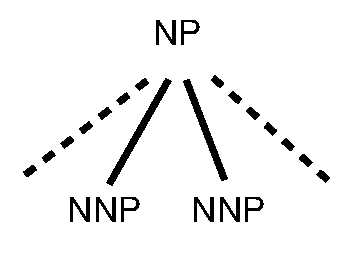
\includegraphics[width=50mm]{dia/people.eps}
	\caption{People extraction tree pattern}
	\label{fig:people-extraction}
\end{figure}

Fig. \ref{fig:people-extraction} shows the sub-tree relating to singular proper nouns (NNP) nodes, from where people involved in the event can be extracted. As the phrasal structure does not allow for easy extraction of this information (this structure alone can not infer if the proper nouns refer to a country or a name or even a brand), a sentence is only considered to refer to a person or people only when an NP (noun phrase) node has at least two contiguous NNP child nodes. This leads to the extraction of not only people but also entities and some cities or countries, like ``High Court'' or ``Santa Barbara''.

\newpage
\subsection{Location extraction}
\label{subsec:approach:location-extraction}

\begin{figure}[h!]
	\centering
	\subfloat[Location extraction tree pattern 1]{\label{fig:local_1}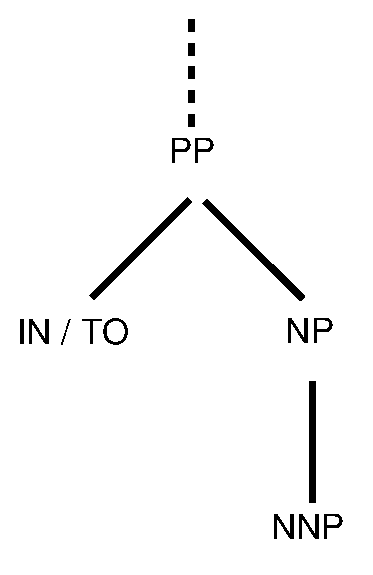
\includegraphics[width=0.3\textwidth]{dia/local_1.eps}}     
	\hspace{20mm}
	\subfloat[Location extraction tree pattern 2]{\label{fig:local_2}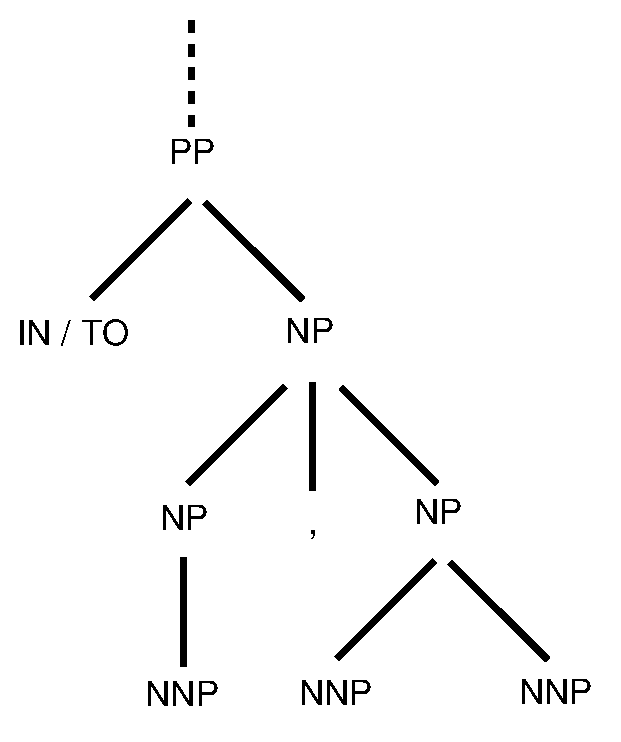
\includegraphics[width=0.4\textwidth]{dia/local_2.eps}}
	\caption{Sub-trees for event location extraction}
	\label{fig:location-extraction}
\end{figure}

Fig. \ref{fig:location-extraction} shows the sub-trees used for extraction the location of the parsed event. A location almost always occurs inside a PP (prepositional phrase) node, and the structure of the descendant nodes determines if it refers to a location, be it a city, a country (Fig. \ref{fig:location-extraction} (a)), or a \textit{complex} location, like a city followed by its country (Fig. \ref{fig:location-extraction} (b)). Although only two main parse tree patterns are presented, the complete list of node sequences used to extract a location is presented in Fig. \ref{fig:nodes-order}.

\begin{figure}[h!]
	\centering
	\begin{tabular}{p{4cm}}
		\begin{verbatim}
		PP - IN - NP - NNP
		PP - TO - NP - NNP
		PP - IN - NP - NP - NNP
		PP - IN - NP - DT - NNPS
		PP - TO - NP - NP - NNP
		PP - IN - NP - DT - NNP
		\end{verbatim}
	\end{tabular}
	\caption{Order of nodes used to recognize locations in sentences}
	\label{fig:nodes-order}
\end{figure}

In addition, when a valid location for the event is found, a request is made to Google HTTP Geocoding Services\footnote{http://code.google.com/apis/maps/documentation/geocoding/index.html} in order to determine the latitude and longitude for that location.

\section{Results}

\subsection{Text Classification}

Using the naive Bayes classifier implementation by Lucas Carlson and David Fayram II\cite{classifier} it was possible to classify the extracted events in the seven categories referred in section \ref{subsec:approach:text-classification}. The accuracy of this classification is shown on Fig. \ref{fig:classifier-accuracy}.

\subsubsection{Metodology}

Ten test runs were made in order to assess the accuracy of the classifier implementation used: from the 350 manually classified examples, 315 were extracted for classification and 35 for testing. The test samples were not included in the classification. Each of the test runs used different samples for classification and testing from the previous runs. Accuracy is defined as
\begin{figure}
	\centering
	\Large{$accuracy = \frac{correct\ results}{sample\ size}$}
	\caption{Classification accuracy definition}
\end{figure}

\subsubsection{Results}

%\begin{figure}[h!]
%	\centering
%	\begin{tabular}{c|c|c}
%		 & \textbf{correctly classified as} & \textbf{incorrectly classified as} \\
%		\hline
%		\textbf{Accidents} & 19 & 4 \\
%		\textbf{Crime}     & 14 & 5 \\
%		\textbf{Cultural}  & 12 & 2 \\
%		\textbf{Economy}   & 5 & 16 \\
%		\textbf{Politics}  & 29 & 1 \\
%		\textbf{Science}   & 12 & 7 \\
%		\textbf{War}       & 10 & 7 \\
%		\hline
%		\textbf{Total}     & 103 & 42 \\
%	\end{tabular}
%	\caption{Accuracy of events classification using a naive Bayes classifier}
%	\label{fig:classifier-accuracy}
%\end{figure}
\begin{figure}[h!]
	\centering
	\begin{tabular}{c|c|c|c}
	\textbf{Test Run} & \textbf{Correct} & \textbf{Incorrect} & \textbf{Accuracy}\\
	\hline
	1 & 21 & 14 & 60.0\% \\
	2 & 22 & 13 & 62.9\% \\
	3 & 29 & 6 & 82.9\% \\
	4 & 25 & 10 & 71.4\% \\
	5 & 23 & 12 & 65.7\% \\
	6 & 26 & 9 & 74.3\% \\
	7 & 20 & 15 & 57.1\% \\
	8 & 20 & 15 & 57.1\% \\
	9 & 27 & 8 & 77.1\% \\
	10 & 21 & 14 & 60\% \\
	\hline
	Total & 234 & 116 & 66.8 \%
	\end{tabular}
	\caption{Accuracy of events classification using a naive Bayes classifier}
	\label{fig:classifier-accuracy}
\end{figure}

From a total of 10 test runs, 234 out of 350 events were correctly classified, yielding an accuracy of 66.8\%. However, some of the events are difficult even for humans to classify, bringing the expected classification accuracy of a larger test set to be between 70\%-75\%. It must be noted that there is a very fine line between economic and political events, which may lead to some bias towards the political side in the training set.

\subsection{Entities Extraction}

The techniques described in sections \ref{subsec:approach:nlp}, \ref{subsec:approach:entities-extraction}, \ref{subsec:approach:location-extraction} allow the extraction of features from sentences. The accuracy of these techniques is shown in Fig. \ref{fig:feature-extraction-accuracy}.

\begin{figure}[h!]
	\centering
	\begin{tabular}{c|c|c}
		& \textbf{Location Extraction} & \textbf{People Extraction} \\
		\hline
		\textbf{Correct}   & 96 & 105 \\
		\textbf{Incorrect} & 49 & 40 \\
		\hline
		\textbf{Accuracy}  & 66\% & 72\% \\ 
	\end{tabular}
	\caption{Accuracy of feature extraction using natural language processing}
	\label{fig:feature-extraction-accuracy}
\end{figure}

This evaluation was performed with these criteria:

\begin{itemize}
	\item If an event does not contain any people and no people are detected, it is considered a successful extraction
	\item If an event does not refer to a location and no location is found, it is construed a successful extraction
	\item If more than one ``person'' is detected and one of them is a person to whom the event refers (even if the other people are not human, but stadiums or countries with more than 2 proper nouns), it is considered a successful extraction\footnote{A collective person, e.g. ``Israeli Air Force'' is considered to be correct if extracted} \footnote{An animal baptized with a name is also considered as ``people'', in regards to what is considered a successful extraction}
	\item All other cases result in an unsuccessful extraction
\end{itemize}

\section{Final Remarks}

The main objectives of the text mining applied in this project were fulfilled. Text classification results could be improved by using a larger and a less biased training set. However, for a training set this size, the results are quite acceptable. Feature extraction using natural language processing can also be considered successful as location and people involved in the majority of the events were successfully extracted. However, a more detailed analysis of the phrasal structures could be the key to less ``noise'' when extracting these informations.

\subsection{Main implementation problems}

Wikipedia is an open knowledge base, relying mainly on user generated content. As such, it is difficult to ensure a proper and constant textual structure for information. Although the pages for the most recent centuries (approx. 18th century) have a well defined an constant HTML structure that allows for reliable information retrieval, there are many years that do not follow this structure, leading to specific parsing cases.\\

This openness lead to another problem: an HTML structure not suited for easy parsing. A series of workarounds had to be implemented to successfully extract useful information.

\newpage
%
% ---- Bibliography ----
%
\begin{thebibliography}{}
%
\bibitem[1]{santorini}
Santorini, B. :
Part-of-Speech Tagging Guidelines for the
Penn Treebank Project (3rd Revision, 2nd Printing).
(July 1990)

\bibitem[2]{bies}
Bies, A., Ferguson, M., Katz, K., MacIntyre, R. :
Bracketing Guidelines for Treebank II
Penn Treebank Project
(June 1995)

\bibitem[3]{classifier}
Carlson, L., Fayram II, D.
http://classifier.rubyforge.org/
(September 2005)

\bibitem[4]{sp}
Stanford University
http://nlp.stanford.edu/software/lex-parser.shtml
(July 2009)

\bibitem[5]{russel}
Artificial Intelligence: A Modern Approach (2nd Edition)
Russel, S., Norvig, P.
(2003)

\end{thebibliography}

\end{document}
